\documentclass[aspectratio=169]{beamer}

% Themes that you can uncomment it to use
% How to see what themes on your computer that you can use
% The following cpmmand may help you:
%
% ls /usr/share/texlive/texmf-dist/tex/latex/beamer | grep "^beamertheme"
%
% Or you can go to:
% https://deic.uab.cat/~iblanes/beamer_gallery/   to see more info

%%%%%%%%%%%%%%%%%%%%%%%%%%%%%%%%%%%%%%%%
% User defined color 
% you can also get more from http://latexcolor.com/
%%%%%%%%%%%%%%%%%%%%%%%%%%%%%%%%%%%%%%%%
\definecolor{mygreen}{rgb}{.125, .5, .25}

%%%%%%%%%%%%%%%%%%%%%%%%%%%%%%%%%%%%%%%%
% \usetheme[named=mygreen]{Berkeley}
% \usetheme{Warsaw}
 \usetheme{metropolis} % reference:https://mirror.mwt.me/ctan/macros/latex/contrib/beamer-contrib/themes/metropolis/doc/metropolistheme.pdf
% \usetheme{AnnArbor}
% \usetheme{Berlin}
%%%%%%%%%%%%%%%%%%%%%%%%%%%%%%%%%%%%%%%%

%%%%%%%%%%%%%%%%%%%%%%%%%%%%%%%%%%%%%%%%
% \usecolortheme{crane}
% \usecolortheme{seahorse}
% \usecolortheme{dolphin}
%%%%%%%%%%%%%%%%%%%%%%%%%%%%%%%%%%%%%%%%


%%%%%%%%%%%%%%%%%%%%%%%%%%%%%%%%%%%%%%%%
% support for chinese
%%%%%%%%%%%%%%%%%%%%%%%%%%%%%%%%%%%%%%%%
\usepackage{ctex}

%%%%%%%%%%%%%%%%%%%%%%%%%%%%%%%%%%%%%%%%
% support for images and set the image path
%%%%%%%%%%%%%%%%%%%%%%%%%%%%%%%%%%%%%%%%
\usepackage{graphicx}
\graphicspath{ {./images/} }


%%%%%%%%%%%%%%%%%%%%%%%%%%%%%%%%%%%%%%%%
% support for table
%%%%%%%%%%%%%%%%%%%%%%%%%%%%%%%%%%%%%%%%
\usepackage{multirow}



\begin{document}
%
% Basic Information Of This Silde
%

\title{计算机素质基础|深圳市考 | 安徽计算机专业测试}
\author{小刘}
\institute{公考89}
\date{\today}




%%%%%%%%%%%%%%%%%%%%%%%%%%%%%%%%%%%%%%%%
% titlepage
%%%%%%%%%%%%%%%%%%%%%%%%%%%%%%%%%%%%%%%%
\begin{frame}
\titlepage
\end{frame}

%%%%%%%%%%%%%%%%%%%%%%%%%%%%%%%%%%%%%%%%
% A frame
%%%%%%%%%%%%%%%%%%%%%%%%%%%%%%%%%%%%%%%%
\begin{frame}[t]{1. 计算机基础知识} \vspace{20pt}
    1.1 计算机的发展

    \begin{enumerate}
        \item{世界上第一台计算机 ENIAC, 1946 年 2 月诞生于美国。}
            发展阶段:
        \item{第一代为 1946-1957 年,电子管计算机:数据处理;}
        \item{第二代为 1958-1964 年,晶体管计算机:工业控制;}
        \item{第三代为 1965-1971 年,中小规模集成电路:小型计算机;}
        \item{第四代为 1972 迄今,大规模和超大规模集成电路:微型计算机;}
            CPU:
        \item{1971 年 Intel 公司开发出 Intel 4004(第一块 CPU)微处理器,标志进入了微型
机阶段。}\\
\textbf{电子 -> 晶体 -> 中小集成 -> 大规模集成}

    \end{enumerate}

\end{frame}


%%%%%%%%%%%%%%%%%%%%%%%%%%%%%%%%%%%%%%%%
% A frame
%%%%%%%%%%%%%%%%%%%%%%%%%%%%%%%%%%%%%%%%
\begin{frame}[t]{1. 计算机基础知识} \vspace{20pt}
    1.2 我国计算机的发展

    \begin{enumerate}
        \item{1958 年 我国研制成功第一台计算机 103 机;}
        \item {1983 年 国防科技大学研制成功的银河-I 号亿次运算巨型计算机是我国自行研制的
第 1 台亿次运算计算机系统;
}
        \item {2009 年 曙光 5000A,峰值计算速度超过 200 万亿次(我国首台百万亿次超级计算机);}
        \item {2009 年 11 月 “天河一号”的峰值速度达到每秒 1206.19 万亿次,是中国首台每秒运
算速度超过千万亿次的超级计算机。
}
        \item {2010 年 “天河一号”升级后的“天河一号 A” 的峰值速度达到每秒 2570 万亿次,
速度超过当时的最快的超级计算机—美国的“美洲豹”(每秒 1750 万亿次),
成为当时世界上运算速度最快的计算机。}
    \end{enumerate}

\end{frame}

%%%%%%%%%%%%%%%%%%%%%%%%%%%%%%%%%%%%%%%%
% A frame
%%%%%%%%%%%%%%%%%%%%%%%%%%%%%%%%%%%%%%%%
\begin{frame}[t]{1. 计算机基础知识} \vspace{20pt}
    1.3 计算机的分类

    \begin{enumerate}
        \item{按用途分}\\
            通用计算机\\
            专用计算机\\
        \item{按规模及性能分} \\
            巨型计算机\\
            大/中型计算机\\
            小型计算机\\
            微型计算机\\
            工作站和服务器。\\
        \item{ 按计算机的原理分类:模拟式电子计算机、数字电子计算机和数字模拟混合式电子计算机}
    \end{enumerate}

\end{frame}

%%%%%%%%%%%%%%%%%%%%%%%%%%%%%%%%%%%%%%%%
% A frame
%%%%%%%%%%%%%%%%%%%%%%%%%%%%%%%%%%%%%%%%
\begin{frame}[t]{1. 计算机基础知识} \vspace{20pt}
    1.4 计算机的特点
            自动控制能力;\\
            处理速度快、精度高;\\
            “记忆”能力强;\\
            能进行逻辑判断;\\
            很高的计算精度;\\
            支持人机交互;通用性强。\\
            支持人机交互;通用性强。\\
            计算机的体系结构仍在继续发展,其发展趋势是智、多、网、巨、微。\\
\end{frame}

%%%%%%%%%%%%%%%%%%%%%%%%%%%%%%%%%%%%%%%%
% A frame
%%%%%%%%%%%%%%%%%%%%%%%%%%%%%%%%%%%%%%%%
\begin{frame}[t]{1. 计算机基础知识} \vspace{20pt}
    1.5 计算机的主要应用领域

    \begin{enumerate}
        \item{科学计算:最早的应用领域}\\ 如导弹的发射,宇宙飞船的飞行轨迹计算等。
        \item{数据处理(信息处理):最广泛的应用领域} 
            \\包括对数据的收集、记载、分类、排序、检索、计算或加工、传输、制 表等工作。
            例如,在科研、生产和经济活动中,把所获得的大量信息存入计算机,通过加工处理,
            得到可供某种目的使用的新信息。
        \item{实时控制}\\ 常用于电力、冶金、石油化工、机械等工业。
        \item{计算机辅助} \\ 计算机辅助设计(CAD);计算机辅助制造(CAM)
            计算机辅助教学(CAI);计算机辅助测试(CAT)
    \end{enumerate}

\end{frame}

%%%%%%%%%%%%%%%%%%%%%%%%%%%%%%%%%%%%%%%%
% A frame
%%%%%%%%%%%%%%%%%%%%%%%%%%%%%%%%%%%%%%%%
\begin{frame}[t]{1. 计算机基础知识} \vspace{20pt}

    练习题\\
        1. 世界上第一台电子计算机诞生于(    )\\
            A. 1945 年\\
            B. 1946 年\\
            C. 1949 年\\
            D. 1950 年\\

\end{frame}

%%%%%%%%%%%%%%%%%%%%%%%%%%%%%%%%%%%%%%%%
% A frame
%%%%%%%%%%%%%%%%%%%%%%%%%%%%%%%%%%%%%%%%
\begin{frame}[t]{1. 计算机基础知识} \vspace{20pt}

    练习题\\
            2. 计算机发展过程按使用的电子器件可划分为四代,微型计算机出现在第( )代。\\
            A. 1\\
            B. 2\\
            C. 3\\
            D. 4\\
\end{frame}


%%%%%%%%%%%%%%%%%%%%%%%%%%%%%%%%%%%%%%%%
% A frame
%%%%%%%%%%%%%%%%%%%%%%%%%%%%%%%%%%%%%%%%
\begin{frame}[t]{1. 计算机基础知识} \vspace{20pt}

    练习题\\
            3. 2009 年 6 月 15 日下午,中国首台国产百万亿次超级计算机,每秒峰值计算
速度超过( )万亿次的曙光 5000A—“魔方”在上海超级计算中心正式启用,这标
志着中国已成为继美国之后的一个研发、制造并部署百万亿次超级计算机的国家。

            A. 100\\
            B. 150\\
            C. 200\\
            D. 250\\
\end{frame}

%%%%%%%%%%%%%%%%%%%%%%%%%%%%%%%%%%%%%%%%
% A frame
%%%%%%%%%%%%%%%%%%%%%%%%%%%%%%%%%%%%%%%%
\begin{frame}[t]{1. 计算机基础知识} \vspace{20pt}

    练习题\\
    4.计算机应用最广泛的领域是( )\\
    A. 科学计算\\
    B. 信息处理\\
    C. 过程控制 \\
    D. 人工智能\\

\end{frame}



%%%%%%%%%%%%%%%%%%%%%%%%%%%%%%%%%%%%%%%%
% A frame 
%%%%%%%%%%%%%%%%%%%%%%%%%%%%%%%%%%%%%%%%
\begin{frame}[t]{2. 计算机系统的组成} \vspace{20pt}

    计算机的组成\\
    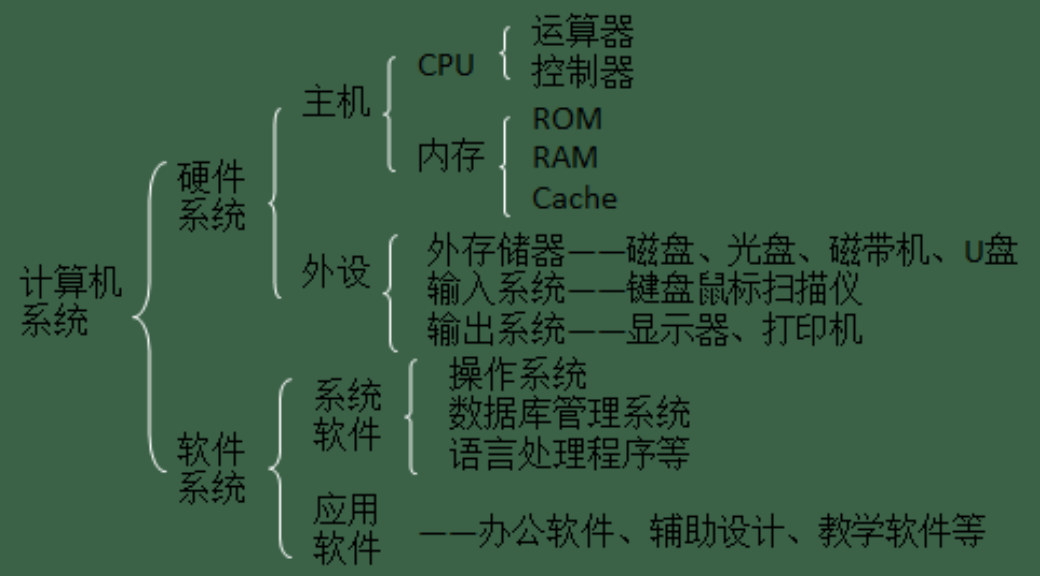
\includegraphics[scale=0.25]{computer_hardware}\\ 
    NOTE: \\
    \textbf{ROM} ||  \textbf{RAM}\\
    \textbf{cache} 
    \textbf{DMA} 
\end{frame}



%%%%%%%%%%%%%%%%%%%%%%%%%%%%%%%%%%%%%%%%
% A frame 
%%%%%%%%%%%%%%%%%%%%%%%%%%%%%%%%%%%%%%%%
\begin{frame}[t]{2. 计算机系统的组成} \vspace{20pt}
    2.1 计算机硬件的概念

    \begin{enumerate}
        \item{计算机硬件(Computer hardware)是指计算机系统中由电子、机械和光电元件等组
            成的各种物理装置的总称}\\
        \item {冯·诺依曼 体系结构}\\
        \item {冯·诺依原理核心思想}\\
            (1)使用二进制;\\
            (2)存储程序和程序控制;\\
            (3)一个完整的计算机硬件系统应该由五个部分组成:运算器、控制器、存储器、
            输入设备、输出设备。\\
    \end{enumerate}

\end{frame}


%%%%%%%%%%%%%%%%%%%%%%%%%%%%%%%%%%%%%%%%
% A frame 
%%%%%%%%%%%%%%%%%%%%%%%%%%%%%%%%%%%%%%%%
\begin{frame}[t]{2. 计算机系统的组成} \vspace{20pt}
    2.2 计算机硬件的各部分功能\\
    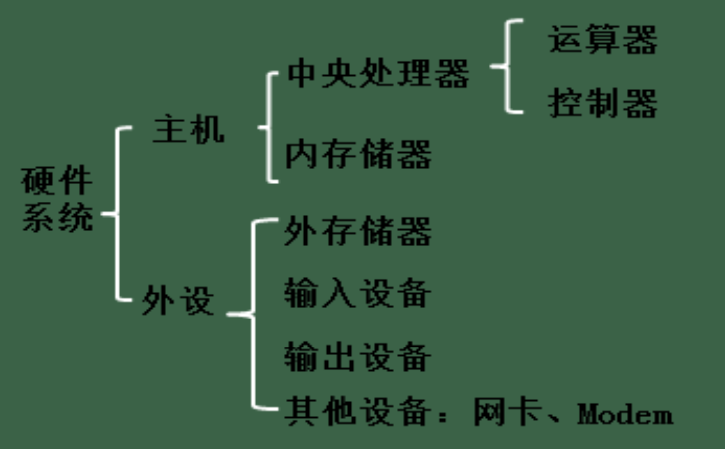
\includegraphics[scale=0.25]{hardware_function}\\ 
\end{frame}

%%%%%%%%%%%%%%%%%%%%%%%%%%%%%%%%%%%%%%%%
% A frame 
%%%%%%%%%%%%%%%%%%%%%%%%%%%%%%%%%%%%%%%%
\begin{frame}[t]{2. 计算机系统的组成} \vspace{20pt}
    2.2 计算机硬件的各部分功能
    \begin{enumerate}
        \item {运算器}\\
            运算器是计算机对数据进行加工处理的中心,对二进制数码进行算术运算或逻辑运
算。\\
计算机的运算速度通常是指每秒钟能够执行加法指令的数目。通常用百万次/每秒
(MIPS)来表示。\\

\item {控制器:}\\
    控制器是计算机的控制中心,由它指挥各个部件自动、协调地工作。\\

    \textbf{运算器 + 控制器 = 中央处理器(CPU)}

\item {存储器:}\\
    存储器是计算机中存放所有数据和程序的记忆部件,它的基本功能是按指定的地址存
(写)入或者取(读)出信息。\\


    \end{enumerate}
\end{frame}


%%%%%%%%%%%%%%%%%%%%%%%%%%%%%%%%%%%%%%%%
% A frame 
%%%%%%%%%%%%%%%%%%%%%%%%%%%%%%%%%%%%%%%%
\begin{frame}[t]{2. 计算机系统的组成} \vspace{20pt}
\textbf{换算关系:}\\
字节、字、位、比特,这四者之间的关系是:\\

    1位=1比特(bit)\\
    1字节(byte)=8位(bit)\\
    1字=2字节(byte)\\
    1字=16位(bit)\\ 

    01|11|00|01||01|01|01|00\\
    0:===================> 1位/1比特 (bit)\\
    01|11|00|01:=============> 1 字节(byte) = 8 比特(bit)\\
    01|11|00|01||01|01|01|00 :======> 1 字 = 2 字节(byte) = 16 位(bit)\\
\end{frame}



%%%%%%%%%%%%%%%%%%%%%%%%%%%%%%%%%%%%%%%%
% A frame 
%%%%%%%%%%%%%%%%%%%%%%%%%%%%%%%%%%%%%%%%
\begin{frame}[t]{2. 计算机系统的组成} \vspace{20pt}
    \textbf{ROM || RAM || CACHE}\\
    a)只读存储器(ROM):是一种只能读出事先所存数据的固态半导体存储器。其特性
是一旦储存资料就无法再将之改变或删除。通常用在不需经常变更资料的电子或电脑
系统中,并且资料不会因为电源关闭而消失。\\
b)随机存储器(RAM):可以被 CPU 随机地读写,故又称为读写存储器。这种存储器
用于存放用户装入的程序、数据及部分系统信息。当机器断电后,所有信息全部丢失。\\
c)高速缓冲存储器(CACHE):用于临时存储频繁使用的信息以加快访问速度。在计
算机存储系统的层次结构中,介于中央处理器和主存储器之间的高速小容量存储器。\\

\textit{外存储器(辅助存储器):简称外存或副存。CPU 不可直接访问其的数据,只
有先调入内存方可使用。例如:硬盘、U 盘、光盘、软盘}\\
\end{frame}


%%%%%%%%%%%%%%%%%%%%%%%%%%%%%%%%%%%%%%%%
% A frame 
%%%%%%%%%%%%%%%%%%%%%%%%%%%%%%%%%%%%%%%%
\begin{frame}[t]{2. 计算机系统的组成} \vspace{20pt}
    
    4.输入设备:\\
    功能:\\
    向计算机输入命令、程序、数据等信息。把这些信息转换为计算机能识别的二
进制代码。\\

例子:\\
    键盘、鼠标、扫描仪、手写板、麦克、照相机、摄像机、游戏操作杆、条形码
阅读器、光学字符阅读器、触摸屏、光笔等。\\

5.输出设备\\
功能:将计算机处理后的各种内部格式信息转换为人们能识别的形式表达出来。\\
例子:显示器、打印机、绘图仪、音响等。\\
\end{frame}


%%%%%%%%%%%%%%%%%%%%%%%%%%%%%%%%%%%%%%%%
% A frame 
%%%%%%%%%%%%%%%%%%%%%%%%%%%%%%%%%%%%%%%%
\begin{frame}[t]{2. 计算机系统的组成} \vspace{20pt}
    2.3 微型计算机的主要技术指标\\
    \begin{enumerate}
        \item{字长:CPU 一次能同时处理二进制数据的位数。}\\
        \item{.时钟主频:指 CPU 的时钟频率,单位 GHz。}\\
            主频=外频*倍频\\
        \item{运算速度:指每秒钟所能执行加法指令数目,常用 MIPS 表示。}\\
        \item{存储容量:主要指内存的存储容量。}\\
        \item{存取周期:指 CPU 从内存储器中存取数据所需要的时间。}\\

    \end{enumerate}

\end{frame}




%%%%%%%%%%%%%%%%%%%%%%%%%%%%%%%%%%%%%%%%
% A frame 
%%%%%%%%%%%%%%%%%%%%%%%%%%%%%%%%%%%%%%%%
\begin{frame}[t]{2. 计算机系统的组成} \vspace{20pt}
    练习题\\
    【单选】1. 冯 · 诺依曼理论的核心是存储程序和( )\\
    A. 顺序存储\\ B. 程序控制\\
    C. 集中存储\\ D. 运算存储分离\\


\end{frame}



%%%%%%%%%%%%%%%%%%%%%%%%%%%%%%%%%%%%%%%%
% A frame 
%%%%%%%%%%%%%%%%%%%%%%%%%%%%%%%%%%%%%%%%
\begin{frame}[t]{2. 计算机系统的组成} \vspace{20pt}
    练习题\\
    【多选】计算机在工作过程中突然断电,不会丢失所保存信息的存储介质是( )\\
    A. 光盘 \\
    B. 硬盘\\
    C. 只读存储器\\
    D. 内存\\
    答案:ABC\\


\end{frame}


%%%%%%%%%%%%%%%%%%%%%%%%%%%%%%%%%%%%%%%%
% A frame 
%%%%%%%%%%%%%%%%%%%%%%%%%%%%%%%%%%%%%%%%
\begin{frame}[t]{2. 计算机系统的组成} \vspace{20pt}
    练习题\\
    【单选】微机中 1K 字节表示的二进制位数是( )\\
A. 1000\\
B. 8×1000\\
C. 1024\\
D. 8×1024\\
\end{frame}



%%%%%%%%%%%%%%%%%%%%%%%%%%%%%%%%%%%%%%%%
% A frame 
%%%%%%%%%%%%%%%%%%%%%%%%%%%%%%%%%%%%%%%%
\begin{frame}[t]{2. 计算机系统的组成} \vspace{20pt}
    练习题\\
    【单选】微机中 1K 字节表示的二进制位数是( )\\
A. 1000\\
B. 8×1000\\
C. 1024\\
D. 8×1024\\
1k = 1024 字节 = 8 * 1024 字/bit/比特/二进制位数\\
答案:D\\
\end{frame}


%%%%%%%%%%%%%%%%%%%%%%%%%%%%%%%%%%%%%%%%
% A frame 
%%%%%%%%%%%%%%%%%%%%%%%%%%%%%%%%%%%%%%%%
\begin{frame}[t]{2. 计算机系统的组成} \vspace{20pt}
    练习题\\
    【多选】 下列属于输入设备的是( )\\
    A. 鼠标\\ B. 打印机\\
    C. 扫描仪\\ D. 显示器\\
    答案:AC\\
\end{frame}



%%%%%%%%%%%%%%%%%%%%%%%%%%%%%%%%%%%%%%%%
% A frame 
%%%%%%%%%%%%%%%%%%%%%%%%%%%%%%%%%%%%%%%%
\begin{frame}[t]{3. 计算机软件的概念及分类} \vspace{20pt}
    3.1. \textbf{概念}\\
    计算机软件(Computer Software)是指计算机系统中的程序、数据及其文档。软
件是用户与硬件之间的接口界面。用户主要是通过软件与计算机进行交流。
\end{frame}




%%%%%%%%%%%%%%%%%%%%%%%%%%%%%%%%%%%%%%%%
% A frame 
%%%%%%%%%%%%%%%%%%%%%%%%%%%%%%%%%%%%%%%%
\begin{frame}[t]{3. 计算机软件的概念及分类} \vspace{20pt}
    3.2. \textbf{软件的分类}\\
    |\\
    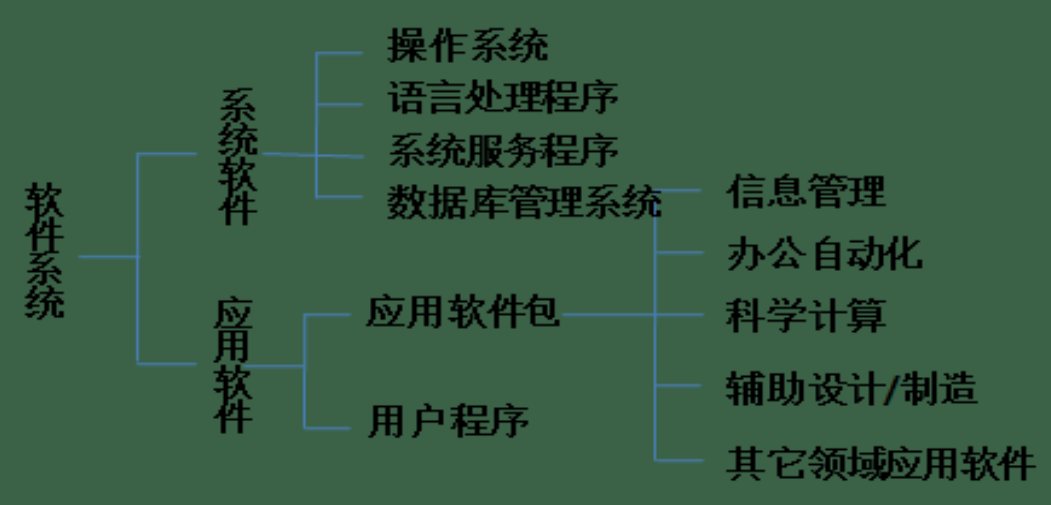
\includegraphics[scale=0.3]{computer_software}\\ 
\end{frame}


%%%%%%%%%%%%%%%%%%%%%%%%%%%%%%%%%%%%%%%%
% A frame 
%%%%%%%%%%%%%%%%%%%%%%%%%%%%%%%%%%%%%%%%
\begin{frame}[t]{3. 计算机软件的概念及分类} \vspace{20pt}
    \begin{enumerate}
        \item{系统软件}\\
            指控制和协调计算机及外部设备,支持应用软件开发和运行的系统,是无需用户干
预的各种程序的集合,主要功能是调度,监控和维护计算机系统;负责管理计算机系
统中各种独立的硬件,使得它们可以协调工作。\\

        \item{应用软件}\\
            在计算机硬件和系统软件的支持下,为解决各类专业和实际问题而设计开发的一
类软件。如杀毒软件、文字处理、电子表格、多媒体制作工具、各种工程设计和数学
计算软件、模拟过程、辅助设计和管理程序等。\\
        \item{程序设计语言}: 人们让计算机完成某项任务的语言\\
            1)机器语言:直接执行\\
2)汇编语言:符号语言,需要编译才能执行\\
3)高级语言:接近自然语言(编译方式和解释方式执行)\\
    \end{enumerate}

\end{frame}

%%%%%%%%%%%%%%%%%%%%%%%%%%%%%%%%%%%%%%%%
% A frame 
%%%%%%%%%%%%%%%%%%%%%%%%%%%%%%%%%%%%%%%%
\begin{frame}[t]{3. 计算机软件的概念及分类} \vspace{20pt}
    练习题:\\
    【多选】下列选项中属于系统软件的是( )\\
A. 数据库管理系统\\ B. 操作系统\\
C. 语言处理系统\\ D. 用户应用程序\\
答案:ABC\\
\end{frame}



%%%%%%%%%%%%%%%%%%%%%%%%%%%%%%%%%%%%%%%%
% A frame 
%%%%%%%%%%%%%%%%%%%%%%%%%%%%%%%%%%%%%%%%
\begin{frame}[t]{3. 计算机软件的概念及分类} \vspace{20pt}
    练习题:\\
    【单选】计算机软件系统包括( )\\
A.系统软件和应用软件\\
B. 编辑软件和应用软件\\
C. 数据库软件和工具软件\\
D. 程序和数据\\
答案:A\\
\end{frame}

%%%%%%%%%%%%%%%%%%%%%%%%%%%%%%%%%%%%%%%%
% A frame 
%%%%%%%%%%%%%%%%%%%%%%%%%%%%%%%%%%%%%%%%
\begin{frame}[t]{4. 计算机中常用的数制及相互转换} \vspace{20pt}
    \textbf{数制基本概念:}\\
    数的表示规则。通常按进位原则进行计数。称为进位计数制,简称数制。人们通
    常采用的数制有十进制、二进制、八进制和十六进制。数制的表示主要包括三个基本
    要素:数码、基数和位权。\\

    \textbf{数码:}是指数制中表示基本数值大小的不同数字符号。\\
    \textbf{基数:}是指数制所使用数码的个数。如 R 进制表示有 R 个基本符号,其基数就为 R。\\
    \textbf{位权:}是指数制中某一位上的 1 所表示数值的大小。\\ 
\end{frame}


%%%%%%%%%%%%%%%%%%%%%%%%%%%%%%%%%%%%%%%%
% A frame 
%%%%%%%%%%%%%%%%%%%%%%%%%%%%%%%%%%%%%%%%
\begin{frame}[t]{4. 计算机中常用的数制及相互转换} \vspace{20pt}

    \begin{tabular}{ |p{2cm}|p{1cm}|p{5cm}|p{1cm}|p{3cm}|  }
        \hline
        \multicolumn{5}{|c|}{数制} \\
        \hline
        进位制  & 基数 & 基本符号(数码)& 权 & 表示\\
        \hline
        二进制  & 2    &     0、1 &                                               2  & B (Binary)\\
        八进制  & 8    &     0、1、2、3、4、5、6、7 &                             8  & O(Octal)\\
        十进制  & 10   &     0、1、2、3、4、5、6、7、8、9 &                       10 & D(Decimal)\\
        十六进制& 16   &     0、1、2、3、4、5、6、7、8、9、A、B、C、D、E、C、F &  16 & H (Hexadecimal)\\
        \hline
    \end{tabular}




\end{frame}


%%%%%%%%%%%%%%%%%%%%%%%%%%%%%%%%%%%%%%%%
% A frame
%%%%%%%%%%%%%%%%%%%%%%%%%%%%%%%%%%%%%%%%
\begin{frame}[t]{4. 计算机中常用的数制及相互转换} \vspace{20pt}
    进制转换\\

二进制:
... 0011101\\
... 64 32 16 8 4 2 1 \\
... 0  0  1  1 1 0 1\\
... 0+ 0+ 16+8+4+0+1 =29 \\

八进制  \\
... 1  0  3\\
... 64 8 1 \\
... 64+0+3 = 67 \\

十进制..  \\
十六进制..\\


\end{frame}





%%%%%%%%%%%%%%%%%%%%%%%%%%%%%%%%%%%%%%%%
% - frame title
% - list
%%%%%%%%%%%%%%%%%%%%%%%%%%%%%%%%%%%%%%%%
% [option] t,c,b:-> from top in this frame
% at the end you can also config 
% like \vspace{10pt}, means: vertial 10pt
\begin{frame}[t]{这个 frame 的 title} \vspace{20pt}
Hello world
    \begin{enumerate}
        \item{this is item 1}
        \item{这是第二个 item}
        \item{\{frame\}[option], option can be  \\
             t -> top(from top)                 \\
             c -> top(from center by default)   \\
             b -> top(from buttom)              \\

        }
    \end{enumerate}

\end{frame}


%%%%%%%%%%%%%%%%%%%%%%%%%%%%%%%%%%%%%%%%
% A frame
%%%%%%%%%%%%%%%%%%%%%%%%%%%%%%%%%%%%%%%%
\begin{frame}[t]{1. 计算机基础知识} \vspace{20pt}
    1.1 计算机的发展

    \begin{enumerate}
        \item{}
        \item{}
        \item{}
        \item{}
        \item{}
        \item{}
            aaa
        \\
\textbf{电子 -> 晶体 -> 中小集成 -> 大规模集成}

    \end{enumerate}

\end{frame}


\end{document}
